\documentclass{beamer}
\usepackage{graphicx} % Required for inserting images

\usepackage[utf8]{inputenc}
% \usepackage[T1]{fontenc}
\usepackage{lmodern}
\usepackage{amsmath,amssymb}
\usepackage{microtype}
\usepackage{ellipsis}
%\usepackage[ngerman]{babel}
\let\openbox\undefined
\usepackage{mathtools}
% \usepackage{enumitem}
% \setbeamertemplate{itemize items}
% \setbeamertemplate{enumerate item}{(\roman{enumi})}
% \let\openbox\undefined
\usepackage{amsthm}
\usepackage{thmtools}
\usepackage{graphicx}
\usepackage{stmaryrd}
\usepackage{tikz}
\usetikzlibrary{shapes.geometric}
\usetikzlibrary{positioning}
\usepackage{algpseudocode}
\usepackage[absolute,overlay]{textpos}
\usepackage{url}
\usepackage[
backend=biber,
style=numeric,
isbn=false,
url=false,
]{biblatex}
\addbibresource{./references.bib}
\usepackage[normalem]{ulem}
\usepackage{xcolor}
\usepackage{structmech}

\declaretheoremstyle[
    headpunct=,
    spacebelow=2em,
    spaceabove=1em,
    postheadspace=\newline,
    ]{aufgabe}
\declaretheorem[style=aufgabe]{aufgabe}
\numberwithin{equation}{aufgabe}
\addtolength\jot{1ex}

\newtheorem{proposition}{Proposition}
\renewcommand\qedsymbol{$\square$}

\newcommand\R{\mathbb R}
\newcommand\Z{\mathbb Z}
\newcommand\N{\mathbb N}
\newcommand\C{\mathbb C}
\newcommand{\Q}{\mathbb Q}
\newcommand{\F}{\mathbb{F}}
\newcommand{\ass}{\underline{Assume:}  }
\newcommand{\zz}{\underline{t.s.:}  }

\renewcommand{\phi}{\varphi}
\renewcommand{\epsilon}{\varepsilon}

\usetheme[compress]{Berlin}
\setbeamertemplate{footline}[frame number]{}
\setbeamertemplate{navigation symbols}{}
\setbeamertemplate{footline}{}

\makeatletter
\beamer@theme@subsectionfalse%
\makeatother

\title{Mechanical Comparison of Arrangement Strategies for Topological Interlocking Assemblies}
\author{Lukas Schnelle \\
This is joint work with Tom Goertzen, Domen Macek, Meike Weiß, Stefanie Reese, Hagen Holthusen and Alice C. Niemeyer \\
Based on \cite{assemblies2023}}
\date{Dec 2023}

\begin{document}

\maketitle

\section{Mathematics}
\begin{frame}{Topological Interlocking}
    \begin{definition}[Topological interlocking assembly]
        A topological interlocking assembly can be defined as an arrangement of blocks that are in contact with each other together with a frame such that, if the frame is fixed, any non-empty finite subset of blocks of the arrangement is prevented from moving.
    \end{definition}
    \pause
    \textbf{Here:} 
    \begin{itemize}
        \item planar topological interlocking assemblies, i.e. between two parallel planes in 3D-space,
        \pause\item use perimeter as the frame,
        \pause\item only copies of the same block differently arranged.
    \end{itemize}  
\end{frame}
\begin{frame}{The Versatile Block}
    The Versatile Block is a polyhedron embedded in $\R^3$, given by \pause vertices 
    $$B_0 \coloneqq \{v_1,\ldots,v_9 \, \},$$ \pause
    edges
    \begin{align*}
        B_1 \coloneqq \{  &\{ v_1, v_2 \},  \{ v_1, v_3 \},  \{ v_1, v_4 \}, \{ v_1, v_5 \}, \{ v_1, v_9 \},  \{ v_2, v_3 \}, \{ v_2, v_5 \}, \\
        & \{ v_2, v_6 \},  \{ v_2, v_7 \},  \{ v_3, v_4 \},  \{ v_3, v_7 \},  \{ v_4, v_7 \}, \{ v_4, v_8 \}, \{ v_4, v_9 \},\\
        & \{ v_5, v_6 \}, \{ v_5, v_7 \},  \{ v_5, v_9 \}, \{ v_6, v_7 \},  \{ v_7, v_8 \},  \{ v_7, v_9 \},  \{ v_8, v_9 \}  \},
    \end{align*} \pause
    and triangular faces
    \begin{align*}
        B_2 \coloneqq \{& \{v_1, v_2, v_3\}, \{v_1, v_2, v_5\},  \{v_1, v_3, v_4\}, \{v_1, v_4, v_9\}, \{v_1, v_5, v_9\}, \\
        &\{v_2, v_3, v_7\},  \{v_2, v_5, v_6\},\{v_2, v_6, v_7\},  \{v_3, v_4, v_7\},  \{v_4, v_7, v_8\},  \\
        &\{v_4, v_8, v_9\},  \{v_5, v_6, v_7\},  \{v_5, v_7, v_9\}, \{v_7, v_8, v_9\}\}.
    \end{align*}
\end{frame}

\begin{frame}{The Versatile Block}
    The Versatile Block is a polyhedron embedded in $\R^3$, given by $B_0, B_1, B_2$ together with coordinates as in \cite{bridges23}
    \begin{alignat*}{3}
    &v_1 = (0, 0, 0) , v_2 = (1, 1, 0) ,  v_3 = (2, 0, 0) , \\
    &v_4 = (1, -1, 0) , v_5 = (0, 1, 1) ,  v_6 = (1, 1, 1) ,  \\
    &v_7 = (1, 0, 1) , v_8 = (1, -1, 1) , v_9 = (0, -1, 1).
    \end{alignat*} 
    \pause
    \begin{center}    
        \includegraphics[width=0.25\textwidth]{images/versatile-front.png}
        \includegraphics[width=0.3\textwidth]{images/versatile-back.png}
        \includegraphics[width=0.33\textwidth]{images/versatile-square.png}
    \end{center}
\end{frame}

\begin{frame}{Isometries}
    \begin{definition}
        Let $n \in \N$, $V$ an euclidean $K$ vectorspace (with metric $d: V \times V \to K$).
        Then $\phi: V \to V$ is called an \emph{isometry} if \pause
        $$
            \forall x, y \in V : d(x, y) = d(\phi(x), \phi(y)).
        $$
    \end{definition}
    \pause
    \textbf{Note:} An isometry is always a combination of an affine transformation and an orthogonal matrix. Such an isometry $\phi = (A, a)$ operates as 
    $$
        (A, a)(x) \coloneqq A \cdot x + a.
    $$
    \pause
    The isometries of a given euclidean vectorspace are a group with the concatenation 
    $$
        \left( (A, a) \circ (B, b) \right) (x) \coloneqq (A \cdot B, A\cdot a + b)
    $$
    denoted by $E(n)$ \pause ($ \implies E(n) = O(n) \ltimes \R^n$).
\end{frame}
\begin{frame}{Wallpaper Groups}
    \begin{definition}[Crystallographic/Wallpaper Groups]
        Let $\Gamma \leq E(n)$ a subgroup of the group of isometries of dimension $n$.\\
        Then $\Gamma$ is called \emph{crystallographic group} if $\Gamma$ is cocompact and discrete, \pause it is called \emph{wallpaper group} if $n=2$.
    \end{definition}
    \pause
    \begin{definition}
        Let $\Gamma \leq E(n)$. \\ \pause
        Then $\Gamma$ is cocompact if the space $E(n) / \Gamma$ is compact.
    \end{definition}
    \pause
    \begin{block}{Proposition (\cite[Prop. 1.9]{szczepanski2012geometry})}
        Let $\Gamma \leq E(n)$. \\
        Then $E(n)/\Gamma$ is compact iff the orbit space $\R^n / \Gamma$ is compact.
    \end{block}
\end{frame}

\begin{frame}{Examples of wallpaper groups}
    \vspace{-3em}
    \begin{alignat*}{2}
    \action<+->{
    &p1 \coloneqq \\
    &\left< 
        \left( \begin{pmatrix} 1 &0 \\ 0 &1\end{pmatrix}, \begin{pmatrix} 1 \\ -1 \end{pmatrix}\right), 
        \left( \begin{pmatrix} 1 &0 \\ 0 &1\end{pmatrix}, \begin{pmatrix} 1 \\ 1 \end{pmatrix}\right) \right> \\ }
    \action<+->{
    &pg \coloneqq \\
    &\left< 
        \left( \begin{pmatrix} 0 &-1 \\ -1 &0\end{pmatrix}, \begin{pmatrix} 2 \\ 0 \end{pmatrix}\right), 
        \left( \begin{pmatrix} 1 &0 \\ 0 &1\end{pmatrix}, \begin{pmatrix} 1 \\ 1 \end{pmatrix}\right) \right> \\ }
    \action<+->{
    &p4 \coloneqq \\
    &\left< 
        \left( \begin{pmatrix} 0 &1 \\ -1 &0\end{pmatrix}, \begin{pmatrix} 0 \\ 2 \end{pmatrix}\right), 
        \left( \begin{pmatrix} 0 &-1 \\ 1 &0\end{pmatrix}, \begin{pmatrix} 0 \\ -2 \end{pmatrix}\right),\left( \begin{pmatrix} -1 &0 \\ 0 &-1\end{pmatrix}, \begin{pmatrix} 0 \\ 0 \end{pmatrix}\right) \right>}
    \end{alignat*}
\end{frame}

\begin{frame}{crystallographic groups on the Versatile Block}
    \begin{center}    
        \includegraphics[width=0.25\textwidth]{images/versatile-front.png}
        \includegraphics[width=0.3\textwidth]{images/versatile-back.png}
        \includegraphics[width=0.33\textwidth]{images/versatile-square.png}
    \end{center}
    \pause
    \textbf{Notice:} Versatile Block has only vertices with $z=0$ and $z=1$.
    Now consider the an isometry $\phi$ from before lifted to $\R^3$ by
    $$
    \hat \phi : \R^3 \to \R^3, \begin{pmatrix}x \\ y \\ z \end{pmatrix} \mapsto  \begin{pmatrix} \phi \begin{pmatrix}x \\ y \end{pmatrix} \\ z \end{pmatrix}
    $$ \pause
    Applied to all coordinates of the vertices of the Versatile Block we get a Versatile Block between the same planes.
\end{frame}

\begin{frame}{Planar Assemblies of the Versatile Block}
    With the groups $p1$, $pg$ and $p4$ from before we get three interlocking assemblies consisting only of copies of the Versatile Block:\\
    \begin{center}
        \only<1-2>{
            \includegraphics[width=0.4\textwidth]{images/p1-rect.png}
            \onslide<2>{
                \includegraphics[width=0.5\textwidth]{images/p1.png}
            }
            \\ \begin{center}
                $p1$
            \end{center}
        }
        \only<3-4>{
            \includegraphics[width=0.4\textwidth]{images/pg-rect.png}
            \onslide<4>{
                \includegraphics[width=0.5\textwidth]{images/pg.png}
            }
            \\ \begin{center}
                $pg$
            \end{center}
        }
        \only<5-6>{
            \includegraphics[width=0.4\textwidth]{images/p4-rect.png}
            \onslide<6>{
                \includegraphics[width=0.5\textwidth]{images/p4.png}
            }
            \\ \begin{center}
                $p4$
            \end{center}
        }
    \end{center}
\end{frame}

\section{Mechanics and Simulation}
\begin{frame}{Problem statement}
    \begin{exampleblock}{Problem}
        Do the $p1$, $pg$ and $p4$ assemblies perform mechanically differently when pressure is applied from one side?\\
    \end{exampleblock}
    \pause
    Setup like this:\\
    \includegraphics[width=0.8\textwidth]{images/setup-10x10.png}
\end{frame}

\begin{frame}{Finite Element Method}
    % \vspace*{-0.5cm}
    How to answer such a question? \pause $\xrightarrow{}$ Finite Element Method\\ \pause
    For now, let us switch to the $\R^2$ case.\\ \pause
    \textbf{Note:} in $\R^2$ there are two (linearly independent) directions of movement and one rotation that classify all movements.
    \pause
    \begin{definition}[Beam]
        A beam is a body in the shape of a cuboid in $\R^2$ that has one dimension much larger than the other two.
    \end{definition}
    \pause
    \begin{definition}[Supports]
        \begin{columns}
        \begin{column}{0.21\textwidth}
            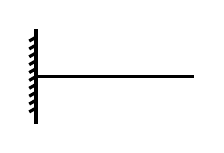
\begin{tikzpicture}
                \draw[line width=0.5mm] (0,0) -- (2,0);
                \FixedSupport[270]{0,0}{1.5}
            \end{tikzpicture}\\
            No rotation or translation.
        \end{column}
        \pause
        \begin{column}{0.3\textwidth}
            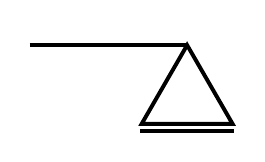
\begin{tikzpicture}
                \node[draw=none] at (2,0.1) {};
                \draw[line width=0.5mm] (0,0) -- (2,0);
                \node[isosceles triangle,
                    isosceles triangle apex angle=60,
                    draw,
                    rotate=90,
                    line width =0.5mm,
                    minimum size =1cm] (T2)at (2,-0.7){};
                \draw[line width=0.5mm] (1.4,-1.1) -- (2.6,-1.1);
            \end{tikzpicture}\\
            Only translation in one direction and rotation.
        \end{column}
        \pause
        \begin{column}{0.3\textwidth}
            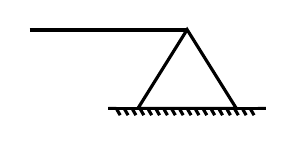
\begin{tikzpicture}
                \draw[line width=0.5mm] (0,0) -- (2,0);
                \HingeSupport[0]{2,0}{2.5}
            \end{tikzpicture}\\
            Only rotation, no translation.
        \end{column}
        \end{columns}
    \end{definition}

\end{frame}

\begin{frame}{Finite Element Method}
    Assumption: Nodes at beams only move in direction of the beam and rotate. \pause
    \begin{enumerate}
        \item Discretization \\ \pause
        Goal: find out how every node is moving in response to the forces applied \pause
        \item Divide and conquer \\ \pause
        There is a possibility to combine the elementary stiffness matrices into a global stiffness matrix \pause
        \item Make an Ansatz \pause
        \item Elementary transfer \\ \pause
        Solve remaining unknowns with principle of minimum potential. \\
        E.g. priciple of virtual work
    \end{enumerate}
\end{frame}

\begin{frame}{Simulation workflow}
    Generate geometries in GAP\\
    \pause $\downarrow$\\
    Generate .stl files from the geometries\\
    \pause $\downarrow$\\
    Convert to .step files \\
    \pause $\downarrow$\\
    Import to Abaqus\\
    \pause $\downarrow$\\
    Set parameters accordingly\\
    \pause $\downarrow$\\
    Run simulation
\end{frame}

\subsection{Simulation Results}
\begin{frame}{Stresses}
    \includegraphics[width=0.9\textwidth]{images/Sm.png}
\end{frame}

\begin{frame}{Deformations}
    \includegraphics[width=0.9\textwidth]{images/u3.png}
\end{frame}

\section{Interlocking Flows}
\begin{frame}{Combinatorial Method}
    \begin{definition}
        Let $A=\{ X_i \mid i\in I\}$, a topological interlocking assembly consisting of blocks $X_i\subset \R^3$ indexed by a finite index set $I$ with a frame indexed by $J\subset I$, the core indexed by $C \coloneqq I \setminus J$ and $d\in \R^3$ a vector.\\ \pause
        The \emph{Directional Blocking Graph} $\mathcal{G}(A,d)$ is defined as the directed graph with \pause
        \begin{itemize}
           \item vertices $I$ and \pause
           \item arcs $i\to j$ if $X_i$ is restrained by $X_j$ in direction $d$ for $i,j\in I$.
        \end{itemize}
    \end{definition}
\end{frame}

\begin{frame}{Combinatorial Method}
    \begin{definition}
        Let $\mathcal{G}(A,d)$ a directional blocking graph of an assembly as before, $i,j \in I$.\\
        Define \pause
        $$v(i\to j) \coloneqq 
            \begin{cases}
                0               & \text{if } (i,j) \notin \mathcal{G}(A,d)\\
                \frac{1}{2},    & \text{if } i\neq j,\\
                1,              & \text{if } i=j.
            \end{cases}$$
        so a block divides the load between the two neighbors of it if it is in the core.
    \end{definition}
    \pause
    Can be viewed as a weighted \emph{adjacency matrix} of $\mathcal{G}$ yielding a flow network with capacity function $v$.
    \pause
    Let $x \in \R^{100}$ a load vector with the amount of force applied to block $i$ in $x_i$.\\ \pause
    For $k$ high enough $A^k \cdot x$ yields the amount of load transferred into the frame.
\end{frame}

\begin{frame}{Combinatorial Results}
    \begin{center}
        \includegraphics[width=0.7\textwidth]{images/flowp1.png}
    \end{center}
\end{frame}

\begin{frame}{Combinatorial Results}
    \begin{center}
        \includegraphics[width=0.7\textwidth]{images/p1-result.png}
    \end{center}
\end{frame}

\begin{frame}{Combinatorial Results}
    \begin{center}
        \includegraphics[width=0.85\textwidth]{images/stress-p1-presentation-top.png}
    \end{center}
\end{frame}

\section{Outlook}
\begin{frame}
    \begin{exampleblock}{Takeaway}
        The arrangement of a topological Interlocking has a high influence on the mechanical performance.
    \end{exampleblock}
    \pause
    Assumptions made:
    \begin{itemize}
        \item Satisfy a wallpaper group \pause$\xrightarrow{}$General Interlocking Assemblies
        \pause
        \item Made from Versatile block \pause $\xrightarrow{}$Made from other blocks
        \pause
        \item Simulations  without friction \pause $\xrightarrow{}$Consider friction
    \end{itemize}
    \pause
    Future work:
    \begin{itemize}
        \item Reduced corners as they often have stress spikes
        \pause
        \item Distance of top and bottom planes
        \pause
        \item Hollow blocks
    \end{itemize}
\end{frame}

\appendix
\begin{frame}    
    Thank you for your attention \bigskip
    \printbibliography 
\end{frame}

\end{document}
